\documentclass[10pt]{article}

\usepackage[a4paper,margin=0.80in]{geometry}
\usepackage{amsmath,amssymb,amsthm,mathtools}
\usepackage{microtype}
\usepackage{booktabs}
\usepackage{tabularx}
\usepackage{enumitem}
\usepackage{xcolor}
\usepackage{tikz}
\usetikzlibrary{arrows.meta,positioning,fit}
\usepackage[colorlinks=true,linkcolor=blue!45!black,
  citecolor=blue!45!black,urlcolor=blue!45!black]{hyperref}

\newtheorem{theorem}{Theorem}
\newtheorem{corollary}[theorem]{Corollary}
\newtheorem{proposition}[theorem]{Proposition}
\theoremstyle{definition}
\newtheorem{definition}[theorem]{Definition}

\newcommand{\C}{\mathbb C}
\newcommand{\R}{\mathbb R}
\newcommand{\N}{\mathbb N}
\newcommand{\Tr}{\operatorname{Tr}}
\newcommand{\ee}{\mathrm e}
\newcommand{\HS}{\mathrm{HS}}
\newcommand{\rank}{\operatorname{rank}}

\title{\textbf{Energy-gap collisions govern quantum recurrence}}
\author{Michael Haufschild}
\date{30 July 2026}

\begin{document}
\maketitle

\begin{abstract}
What determines both when a quantum history returns and how often returns
occur? We identify one spectral variable: collisions among energy
differences. Approximate collisions give a deterministic escape--return law
for every finite energy-sector expectation history and every positive
observational tolerance. Joint optimization over retained coherence
networks and phase resolution defines a least certified post-exit clock;
discarded coherence enters only as distortion. Exact additive collisions
give the complementary law for every probability energy spectrum:
the long-time mean of the \(n\)th power of survival probability equals the
zero mass of the \(n\)-fold convolution of its energy-gap law. Together
these results connect worst-case return time to all long-time survival
moments through the same gap variable. For a localized survival record,
the clock exponent is the number of retained modes inside a localization
ball minus one, exterior modes contribute a controlled spectral tail, and
uniform localization removes ambient system size from the certificate.
The post-exit law extends to every normalized countably infinite pure-point
packet with summable weight and a quadratic phase remainder. Uniform finite
packets supply matching worst-spectrum exponents. Atomless spectra occupy
the opposite boundary: positive-fidelity windows have zero asymptotic time
density. Applied to normalized thermal spectral form factors, the law also
separates what exact global spectral data determine from what an all-orders
perturbative expansion cannot certify.
\end{abstract}

\noindent\textbf{One-sentence summary.}
Approximate energy-gap collisions set how long a quantum return can take;
exact collisions set how often quantum returns occur.

\section*{Energy gaps are the recurrence variable}

Quantum recurrence is usually posed globally: when does a closed state
return near itself? Finite-dimensional unitary dynamics guarantees
arbitrarily accurate returns \cite{BocchieriLoinger1957}; quantitative work
now gives effective-support bounds, post-exit deadlines and simultaneous
all-state estimates \cite{CamposVenuti2015,KotowskiOszmaniec2026,
GuptaShort2026}. Experiments have resolved many-body recurrences
\cite{RauerEtAl2018}, and programmable multiqubit proposals make their
size dependence accessible \cite{KarimiEtAl2026}.

Physical records are rarely global states. A state and an observable select
particular energy gaps \cite{GarciaPintosEtAl2017}; delayed observable
records can reveal a dynamical dimension \cite{WolfPerezGarcia2009}; and
energy-level graphs organize accessible quantum dynamics
\cite{Altafini2002}. These facts suggest a sharper question:
\begin{equation}
 \boxed{\text{Can one spectral law determine both the clock and the
 long-time statistics of quantum return?}}
 \label{eq:question}
\end{equation}
Our answer is the energy-gap law. Its near-zero events have two distinct
meanings. Approximate phase closure of selected gaps determines a finite
resolution return clock. Exact additive cancellation among independent
gaps determines long-time survival moments. The first statement must be
strictly post-exit: a certificate near time zero is physically empty if the
record has not yet left its initial neighbourhood
\cite{KotowskiOszmaniec2026}. The second statement remains meaningful for
finite, countable, continuous and mixed spectra. Localization connects them
to space by limiting the gap information visible to a local survival
measurement.

\begin{figure}[t]
\centering
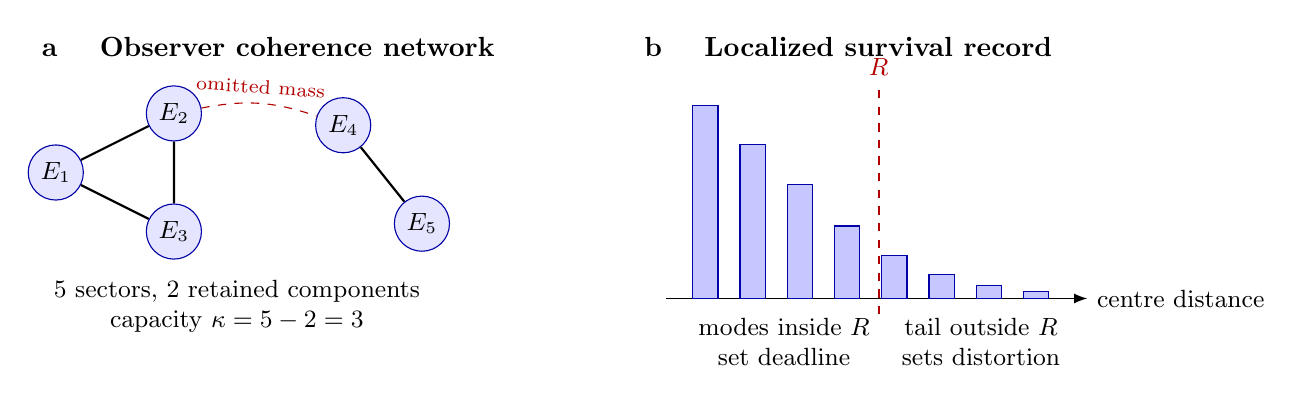
\begin{tikzpicture}[font=\small,>=Latex,
  v/.style={circle,draw=blue!65!black,fill=blue!10,
    minimum size=7mm,inner sep=0pt}]
  \node[anchor=west,font=\bfseries] at (-0.3,3.2)
    {a \quad Observer coherence network};
  \node[v] (a) at (0,1.6) {$E_1$};
  \node[v] (b) at (1.5,2.35) {$E_2$};
  \node[v] (c) at (1.5,0.85) {$E_3$};
  \node[v] (d) at (3.65,2.2) {$E_4$};
  \node[v] (e) at (4.65,0.95) {$E_5$};
  \draw[thick] (a)--(b) (a)--(c) (b)--(c);
  \draw[thick] (d)--(e);
  \draw[dashed,red!70!black] (b) to[bend left=15] node[above,sloped]
    {\scriptsize omitted mass} (d);
  \node[align=center] at (2.3,-0.1)
    {$5$ sectors, $2$ retained components\\capacity $\kappa=5-2=3$};

  \begin{scope}[xshift=8.0cm]
    \node[anchor=west,font=\bfseries] at (-0.65,3.2)
      {b \quad Localized survival record};
    \draw[->] (-0.25,0) -- (5.1,0) node[right] {centre distance};
    \foreach \x/\h in {0.25/2.45,0.85/1.95,1.45/1.45,2.05/0.92,
      2.65/0.55,3.25/0.31,3.85/0.17,4.45/0.09}{
      \fill[blue!22] (\x-0.16,0) rectangle (\x+0.16,\h);
      \draw[blue!65!black] (\x-0.16,0) rectangle (\x+0.16,\h);
    }
    \draw[dashed,red!70!black,thick] (2.45,-0.2) -- (2.45,2.7)
      node[above] {$R$};
    \node[align=center] at (1.25,-0.55)
      {modes inside $R$\\set deadline};
    \node[align=center] at (3.75,-0.55)
      {tail outside $R$\\sets distortion};
  \end{scope}
\end{tikzpicture}
\caption{\textbf{Recurrence as coherence compression.}
\textbf{a}, Retained edges specify relative phases that must synchronize.
One common phase per connected component is invisible, leaving capacity
\(\kappa=|V|-c(G)\). Omitted edges are paid as distortion.
\textbf{b}, For a localized survival record, the retained graph is the
clique on modes centred inside radius \(R\). Its capacity is the number of
inside modes minus one; the exterior spectral tail contributes error.}
\label{fig:law}
\end{figure}

\section*{Approximate collisions: a universal capacity--distortion law}

Let \(V\) be the finite set of distinct energy eigenspaces of a Hamiltonian,
with energies \(E:V\to\R\). A finite family of scalar expectation histories
can be written
\begin{equation}
 f_a(t)=\sum_{K,L\in V}c_a(K,L)\,
   \ee^{\,\mathrm i t(E_K-E_L)},\qquad a\in J.
 \label{eq:history}
\end{equation}
No distinct-gap assumption is made: terms with the same Bohr frequency may
cancel in the sum. Give the records nonnegative weights \(\lambda_a\), and
measure their total displacement by
\begin{equation}
 D(t)=\sum_{a\in J}\lambda_a|f_a(t)-f_a(0)|.
 \label{eq:deviation}
\end{equation}

Choose any undirected graph \(G\) on \(V\). It is a compression choice, not
an assumption about the Hamiltonian. Define cancellation-resistant ordered
pair masses
\[
 m_{KL}=\sum_a\lambda_a|c_a(K,L)|
\]
and
\begin{align}
 M_G&=\sum_{\substack{(K,L)\in V^2\\K\sim_G L}}m_{KL},
 \label{eq:selected}\\
 M_{\bar G}&=\sum_{\substack{(K,L)\in V^2\\K\ne L,\ K\not\sim_G L}}m_{KL}.
 \label{eq:omitted}
\end{align}
Both sums are directed: \(m_{KL}\) and \(m_{LK}\) are separate terms.
Let \(c(G)\) denote the number of connected components, including isolated
vertices, and put
\begin{equation}
 \kappa(G)=|V|-c(G),\qquad
 B_G(Q)=2M_{\bar G}+\frac{4\pi}{Q+1}M_G.
 \label{eq:budget}
\end{equation}

For a target deviation \(\varepsilon\), remove the arbitrary graph choice
by defining the \emph{observable recurrence capacity}
\begin{equation}
 {\cal C}_{\varepsilon}(Q)=
 \min_{\substack{G\\B_G(Q)\le\varepsilon}}\kappa(G),
 \label{eq:optimal-capacity}
\end{equation}
whenever the feasible set is nonempty. The minimum exists because the
sector set is finite. It is a property of the Hamiltonian--record family at
the stated resolution and distortion, not of a preferred basis or a graph
selected after the fact.
The complete graph becomes feasible for every \(\varepsilon>0\) when \(Q\)
is large enough. Jointly optimizing resolution and graph therefore defines
the least certified clock
\begin{equation}
 {\cal T}_{\varepsilon}=
 \min_{\substack{Q\in\N,\ G\\B_G(Q)\le\varepsilon}}
 (Q+1)^{\kappa(G)}.
 \label{eq:optimal-clock}
\end{equation}

\begin{theorem}[Approximate-collision escape--return law]
\label{thm:master}
For every finite energy-sector family, every finite expectation-history
family \eqref{eq:history}, every nonnegative record weighting, every target
\(\varepsilon>0\), and every guard time \(g>0\), one of the following
exhaustive alternatives holds:
\begin{enumerate}[leftmargin=2.2em,label=(\roman*)]
 \item the complete record never exits the guaranteed neighbourhood,
 \[
   D(t)\le \varepsilon\quad\text{for every }t\geq0;
 \]
 \item there is an exit time \(t_{\rm ex}\geq0\) with
 \(D(t_{\rm ex})>\varepsilon\), followed by a return time
 \[
  t_{\rm ret}=n(t_{\rm ex}+g)>t_{\rm ex},
  \qquad
  1\le n\le{\cal T}_{\varepsilon},
  \label{eq:deadline}
 \]
 for which \(D(t_{\rm ret})\le \varepsilon\).
\end{enumerate}
\end{theorem}

The theorem is deterministic and contains no typical-spectrum premise.
Choose a resolution--graph pair attaining \eqref{eq:optimal-clock}.
Synchronizing one spanning forest per retained component requires
\(\kappa(G)\) relative phases; simultaneous approximation supplies the
deadline. Every retained ordered pair then has chord error at most
\(4\pi/(Q+1)\). Every omitted unit-circle chord is at most two, producing
the first term of \eqref{eq:budget}. The never-exits branch is not a defect:
it states that the observer already retains the initial record to the
claimed resolution at all times. Otherwise the theorem certifies a genuine
post-exit return in the same metric.

The quantity \({\cal T}_{\varepsilon}\) is an optimal certified upper clock,
not necessarily the smallest actual return time. Rational relations among
energies can make a fixed Hamiltonian return earlier. We make no matching
lower-bound claim in this scalar record metric for every graph topology.

\subsection*{Basis invariance and physical expectation values}

Let \(P_K\) be the spectral projector onto the eigenspace \(K\), so that
\(\sum_KP_K=I\). For a state \(\rho_a\) and observable \(A_a\), take
\begin{equation}
 c_a(K,L)=\Tr(P_K\rho_aP_LA_a).
 \label{eq:sectorcoeff}
\end{equation}
Then \eqref{eq:history} is exactly
\[
 f_a(t)=\Tr(\rho_a(t)A_a),
\]
and \(f_a(t)-f_a(0)\) is exactly the corresponding trace displacement.
Equation \eqref{eq:sectorcoeff} is invariant under simultaneous changes of
coordinates. Therefore degeneracy cannot change the vertices, masses or
capacity: vertices are eigenspaces, not arbitrarily chosen eigenvectors
inside them.

This correction matters. Entrywise graphs in a chosen energy basis can
change under a rotation within a degenerate eigenspace even though every
physical history remains unchanged. The sector formulation removes that
coordinate artifact while retaining cancellation-safe bounds.

The survival probability provides the common scalar object for the finite
clock and the arbitrary-spectrum law below. For normalized sector weights
\(p_K\ge0\), define
\begin{equation}
 \mu_p=\sum_Kp_K\delta_{E_K},\qquad
 A_{\mu_p}(t)=\int\ee^{itE}\,d\mu_p(E),\qquad
 F_{\mu_p}(t)=|A_{\mu_p}(t)|^2.
 \label{eq:fidelity-measure}
\end{equation}
Its ordered-pair coefficients are \(p_Kp_L\). Thus
\(1-F_{\mu_p}(t)\) is exactly the survival loss controlled by
Theorem~\ref{thm:master}. If \(\Delta\mu_p\) denotes the law of \(E-E'\) for
independent \(E,E'\sim\mu_p\), then \(F_{\mu_p}\) is also exactly the
characteristic function of \(\Delta\mu_p\). Approximate closure of retained
gap phases is therefore the finite-resolution side of one gap law.

The projective exponent cannot be removed in general. For the uniform pure
state on \(r+1\) sectors, scalar survival loss is exactly one half of the
squared Hilbert--Schmidt displacement of its rank-one density matrix.
Explicit spectra avoid a fixed return target through a clock whose
target exponent is \(r\), while every spectrum has a constructive return
with exponent \(r\). This matching statement is for the complete uniform
survival observer; it is not an arbitrary-graph sharpness claim.

\begin{proposition}[Scalar worst-spectrum exponent]
\label{prop:sharp}
Let \(0<\eta\le1\). If
\[
 N(r+1)\exp\!\left(\frac{r+1}{2}\right)
 \left(\sqrt{\frac{\pi\eta}{2}}\right)^r<1,
\]
there is an \((r+1)\)-sector spectrum whose uniform survival loss is
strictly larger than \(1-(1-\eta)^2\) at every integer
\(1\le n\le N\). Conversely, every \((r+1)\)-sector spectrum has some
\[
 1\le n\le(Q+1)^r,\qquad
 1-F_{\mu_p}(n)\le
 2\left(\frac{2\pi}{Q+1}\right)^2.
\]
\end{proposition}

\section*{Localization turns spatial confinement into temporal compression}

The universal theorem becomes a spatial law for a local survival record in
a finite eigensystem. Let a normalized local state have spectral weights
\[
 p_k\geq0,\qquad \sum_kp_k=1,
\]
where \(k\) indexes distinct energy sectors and
\(p_k=\langle x,P_kx\rangle\). Thus degeneracy does not introduce an
eigenbasis choice. In a simple spectrum these sectors are individual
eigenmodes. Define
\begin{equation}
 S_p(t)=\left|\sum_kp_k\ee^{\,\mathrm i tE_k}\right|^2.
 \label{eq:survival}
\end{equation}
The ordered-pair coefficients of \(S_p(t)\) are exactly \(p_kp_l\), and the
record metric is exactly
\[
 |S_p(t)-1|=1-S_p(t).
\]

Assign every retained spectral sector a localization centre certificate and
let \(r_k\in\N\) be its distance from the observed site. For radius \(R\), set
\[
 S_R=\{k:r_k\leq R\},\qquad
 \alpha_R=\sum_{r_k>R}p_k.
\]
Choose the clique on \(S_R\) and leave every exterior mode isolated. Its
capacity is exactly \(|S_R|-1\); selected mass is at most one and omitted
mass is at most \(2\alpha_R\). Consequently, at target
\(\varepsilon^{(1)}_{R,Q}=4\alpha_R+4\pi/(Q+1)\),
\begin{equation}
 {\cal C}_{\varepsilon^{(1)}_{R,Q}}(Q)\le |S_R|-1.
 \label{eq:localized-capacity}
\end{equation}
This is the specialization of the general scalar-history metric. Survival
has a sharper quadratic form. Its exact identity with one half of a
weighted pure-state Hilbert--Schmidt displacement improves the certified
budget to
\begin{equation}
 \varepsilon^{(2)}_{R,Q}=
 4\alpha_R+2\left(\frac{2\pi}{Q+1}\right)^2.
 \label{eq:localized-quadratic-budget}
\end{equation}

\begin{corollary}[Localization-volume escape--return law]
\label{cor:localized}
For every nonempty \(S_R\), resolution \(Q\) and guard time \(g>0\), either
\[
  1-S_p(t)\le\varepsilon^{(2)}_{R,Q}
  \quad\text{for every }t\ge0,
 \label{eq:localized-never}
\]
or an exit from this same neighbourhood is followed by a return satisfying
\begin{align}
  1-S_p(t_{\rm ret})
    &\le\varepsilon^{(2)}_{R,Q},\label{eq:localized-error}\\
  t_{\rm ret}
    &\le(t_{\rm ex}+g)(Q+1)^{|S_R|-1}.
 \label{eq:localized-deadline}
\end{align}
\end{corollary}

The ambient number of energy levels has disappeared. A local record pays
only for modes retained inside its localization ball; everything else is
converted into controlled distortion.

An explicit decay theorem makes this volume independence quantitative.
Suppose
\begin{equation}
 p_k\le C\ee^{-2\mu r_k},\qquad
 \#\{k:r_k=m\}\le AB^m,\qquad
 s:=B\ee^{-2\mu}<1.
 \label{eq:localization}
\end{equation}
Then
\begin{equation}
 0\le\alpha_R\le
 \min\left\{1,\,
 AC\frac{s^{R+1}}{1-s}\right\}.
 \label{eq:tail}
\end{equation}
Combining \eqref{eq:tail} with Corollary~\ref{cor:localized} gives
\begin{equation}
 1-S_p(t_{\rm ret})\le
 4AC\frac{s^{R+1}}{1-s}
  +2\left(\frac{2\pi}{Q+1}\right)^2.
 \label{eq:anderson-error}
\end{equation}
If \(|S_R|\le V_{\rm eff}(R)\), the corresponding deadline is
\((t_{\rm ex}+g)(Q+1)^{V_{\rm eff}(R)-1}\).

The radius and phase resolution can be locked to one scale. Suppose
\(|S_N|\le V(N+1)^\nu\), set \(Q=2^N-1\), and retain the assumptions in
\eqref{eq:localization}. Then the same never-exits or post-exit-return
alternative holds with
\begin{align}
 \varepsilon_N&=
 4AC\frac{s^{N+1}}{1-s}
 +2\left(\frac{2\pi}{2^N}\right)^2,
 \label{eq:scale-error}\\
 n&\le
 2^{\,N\left(V(N+1)^\nu-1\right)}.
 \label{eq:scale-deadline}
\end{align}
Thus observational error falls exponentially in \(N\), while the binary
logarithm of the certified deadline grows as an explicit polynomial of
degree \(\nu+1\). Neither expression contains the ambient number of modes.
This resolution-scale law is the sharpest physical consequence of the
locality transfer: the localization-volume growth exponent controls the
growth class of the local recurrence certificate.

Eigensystem multiscale analysis supplies site-labelled exponentially
localized eigenfunctions for Anderson models in rigorous localization
regimes \cite{ElgartKlein2016,ElgartKlein2018}. Equations
\eqref{eq:localization}--\eqref{eq:anderson-error} state the deterministic
transfer from such eigensystem data to recurrence. They do not constitute a
new proof of Anderson localization, and constants are total-size
independent only when the localization and shell constants are uniform in
volume.

Recurrence and Anderson localization have been linked since the kicked-rotor
mapping of Fishman, Grempel and Prange
\cite{FishmanGrempelPrange1982}. Localized return-to-origin behaviour is
also directly visible in the quantum boomerang effect
\cite{SajjadEtAl2022}. Recent effective-support recurrence bounds already
imply a localization-volume post-exit estimate after inserting an
exponentially localized spectral tail
\cite{KotowskiOszmaniec2026}. Corollary~\ref{cor:localized} is therefore a
quantitative interface between the observer-specific coherence budget used
here and standard localization data; it is not a standalone Anderson
novelty claim.

Anderson localization is normally described as the absence of diffusion
\cite{Anderson1958}. Within the present recurrence framework, exponential
localization compresses finite-resolution observable temporal complexity by
limiting how many spectral phases a local return must coordinate. It need
not reduce exact rational gap rank, because exponentially small overlaps
remain nonzero. Interactions in many-body localized phases can
suppress simple revivals through dephasing
\cite{VasseurParameswaranMoore2015}; our theorem does not reverse that
result. It specifies the deterministic recurrence budget once the visible
spectral tail and effective volume are known.

\section*{Exact collisions: a law for every spectrum}

Let \(\mu\) now be an arbitrary probability measure on \(\R\), with no
assumption of finite support, discreteness or spectral regularity. Define
\begin{equation}
 A_\mu(t)=\int_\R\ee^{itE}\,d\mu(E),\qquad
 F_\mu(t)=|A_\mu(t)|^2,
 \label{eq:general-fidelity}
\end{equation}
and let \(\Delta\mu\) be the law of \(E-E'\) for independent
\(E,E'\sim\mu\). Write
\begin{equation}
 \kappa_n(\mu)=((\Delta\mu)^{*n})(\{0\}),\qquad n\in\N.
 \label{eq:collision-mass}
\end{equation}
The zeroth convolution power is the unit mass at zero.

\begin{theorem}[Universal energy-gap collision law]
\label{thm:collision}
For every probability spectrum \(\mu\):
\begin{enumerate}[leftmargin=2.2em,label=(\roman*)]
 \item \(F_\mu\) is exactly the characteristic function of
 \(\Delta\mu\). Consequently,
 \[
  F_\mu(t)=F_\nu(t)\ \text{for every }t
  \quad\Longleftrightarrow\quad
  \Delta\mu=\Delta\nu .
 \]
 \item A positive-time perfect return \(F_\mu(t)=1\) exists exactly when
 the closed additive group generated by
 \(\operatorname{supp}(\Delta\mu)\) is \(\omega\mathbb Z\) for some
 \(\omega\in\R\).
 \item For every \(n\in\N\),
 \begin{equation}
  \lim_{T\to\infty}\frac1{2T}
    \int_{-T}^{T}F_\mu(t)^n\,dt
  =\kappa_n(\mu).
  \label{eq:collision-law}
 \end{equation}
 Every continuous \(h:[0,1]\to\R\) also has a symmetric-window
 long-time mean when evaluated on \(F_\mu\).
\end{enumerate}
\end{theorem}

The first identity makes the gap law neither a proxy nor a lossy summary:
it is exactly equivalent to the complete survival record. The third identity
turns additive zero-sum gap collisions into every long-time survival moment.
Its \(n=1\) ancestor is Wiener's collision formula \cite{Wiener1933}; the
all-order statement places the entire hierarchy beside the finite
approximate-collision clock. Approximate zero collisions determine
\emph{when} a resolved return is guaranteed; exact zero collisions determine
\emph{how often} returns occur in long-time averages.

\subsection*{Countably infinite survival still has a finite local clock}

For a normalized nonnegative pure-point packet
\[
 p_k\ge0,\qquad \sum_{k=0}^{\infty}p_k=1,
\]
put
\[
 A_\infty(t)=\sum_{k=0}^{\infty}p_k\ee^{it\omega_k},
 \qquad F_\infty(t)=|A_\infty(t)|^2.
\]
For \(M\ge1\), define its exact tail
\(\alpha_M=\sum_{j=0}^{\infty}p_{M+j}\) and budget
\begin{equation}
 B^{\rm surv}_{M,Q}=
 \left(\frac{2\pi}{Q+1}\right)^2
   \sum_{k=1}^{M-1}p_k+4\alpha_M.
 \label{eq:infinite-budget}
\end{equation}

\begin{theorem}[Countably infinite survival escape--return law]
\label{thm:infinite}
For every such packet, every \(M\ge1\), \(Q\in\N\) and \(g>0\), either
\[
 1-F_\infty(t)\le B^{\rm surv}_{M,Q}
 \quad\text{for every }t\ge0,
\]
or an exit is followed strictly later by a return inside the same budget,
with
\[
 1\le n\le(Q+1)^{M-1},\qquad
 t_{\rm ret}=n(t_{\rm ex}+g).
\]
\end{theorem}

Only \(M-1\) projective gaps are synchronized. The complete infinite tail
is retained in \eqref{eq:infinite-budget}; no finite-support replacement of
the state is made. More generally, if \(\alpha_M\le\bar\alpha\) and
\(M\le V\), the same alternative holds after replacing \(\alpha_M\) by
\(\bar\alpha\), with deadline \((Q+1)^{V-1}\). This is the exact
countably infinite localization interface: a proved spectral-tail
certificate supplies distortion, while finite visible volume supplies the
clock.

\section*{Spectral type is the exact recurrence boundary}

Theorems~\ref{thm:collision} and \ref{thm:infinite} do not force one
finite deadline on every spectrum. They identify why that would be false.
Countable pure-point weight can be transferred into a finite head plus an
arbitrarily small tail, producing increasingly accurate finite-resolution
returns. At the opposite endpoint, if \(\mu\) is atomless, then for every
\(\eta>0\) the fraction of the symmetric window \([-T,T]\) on which
\(F_\mu(t)\ge\eta\) tends to zero as \(T\to\infty\). Equivalently, every
positive-order exact collision mass
\(\kappa_n(\mu)\) vanishes. This does not say that an atomless spectrum has
no exceptional returns; it says that positive-fidelity windows occupy zero
fraction of late time.

Mixed spectra are governed without an artificial dichotomy: their atomic
and continuous parts contribute through the single gap measure
\(\Delta\mu\) and its collision masses. Thus the universal statement is not
``everything recurs by one finite clock''. It is:
\begin{center}
\fbox{\parbox{0.86\linewidth}{\centering
The complete survival record, exact return phase and long-time moments all
factor through one energy-gap law.}}
\end{center}

\section*{Global completion is the missing recurrence datum}

Because the complete survival record is equivalent to \(\Delta\mu\),
recurrence is global spectral information. Complete local polynomial data
need not determine it. For every normalized indeterminate Hamburger moment
class there are a pure-point completion and an atomless completion with the
same moment sequence, polynomial Krylov Gram matrix, energy-multiplication
matrix and connected Jacobi rule at every depth, but respectively positive
and zero mean survival recurrence. The construction can be placed on
strictly positive energies
\cite{SalaMayato2020,LoughlinCohen2022,Yafaev2023,BergSzwarc2023}.
Conversely, if one representative of an exact
moment sequence has compact support, exact moments determine the measure
uniquely and therefore determine its complete gap law.

All-orders perturbation has a separate exact obstruction. Let
\(\eta(g)=0\) for \(g\le0\) and \(\eta(g)=\ee^{-1/g}\) for \(g>0\).
On one fixed compact positive interval, an atomless spectral family and the
family obtained by adding an atom of mass \(\eta(g)\) have identical
coupling derivatives at \(g=0\) for every bounded continuous spectral
observable. Their entire time-dependent spectral-form-factor jets also
agree to all orders. Yet for every \(g>0\) their exact mean survival
plateaux are respectively \(0\) and \(\ee^{-2/g}\). Therefore no
model-independent classifier whose only input is either complete jet can
decide whether the plateau is positive.

\subsection*{Thermal spectral form factors and black-hole inference}

For a normalized thermal energy law
\[
 d\mu_\beta(E)=Z(\beta)^{-1}\ee^{-\beta E}\,d\rho(E),
\]
the normalized spectral form factor is exactly
\begin{equation}
 \frac{|Z(\beta+it)|^2}{Z(\beta)^2}=F_{\mu_\beta}(t).
 \label{eq:sff}
\end{equation}
Spectral form factors probe random-matrix behaviour and proposed microscopic
black-hole spectra \cite{BarbonRabinovici2003,CotlerEtAl2017}. Hence
Theorem~\ref{thm:collision} applies without a gravity-specific step: every
long-time thermal survival moment is a zero-sum collision mass of thermal
energy gaps. The perturbative obstruction above gives a sharp certification
boundary. An all-orders coupling expansion of the spectral form factor,
even at every physical time, cannot universally certify a positive exact
plateau; a global nonperturbative spectral completion is required.

This is not a theorem about black-hole microphysics, information recovery,
holography or gravitational dynamics. It states exactly what normalized
thermal spectral data determine and what perturbative spectral data alone
cannot certify.

\section*{Consequences}

The collision law yields four exact separations.
\begin{enumerate}[leftmargin=2.2em]
 \item \textbf{Complete recurrence is gap information.} Two probability
 spectra have the same survival record at every time exactly when their
 energy-gap laws agree. The original energy origin and any other
 phase-retrieval ambiguity beyond the gap law are invisible to recurrence.
 \item \textbf{Ambient size is not the local clock.} Once a localization
 ball, its tail and its volume-growth certificate are fixed, neither
 \eqref{eq:scale-error} nor \eqref{eq:scale-deadline} contains the ambient
 number of energy sectors. The countable theorem removes finite ambient
 support altogether.
 \item \textbf{Global rank cannot bound the first exit.} For every
 nonempty finite site set, every Hermitian hopping matrix, every finite
 horizon \(H\) and every \(\delta>0\), there is a positive coupling and an
 onsite potential with maximal projective spectral rank for which every
 site-survival loss remains below \(\delta\) throughout \([-H,H]\).
 Therefore no universal absolute exit deadline follows from global
 projective rank plus finite-horizon locality. The post-exit formulation is
 mathematically necessary.
 \item \textbf{Exact plateaux require global completion.} Exact moments
 suffice under compact support; complete perturbative jets do not suffice
 universally. Thermal black-hole spectral-form-factor inference inherits
 this same boundary.
\end{enumerate}

The broad interpretation is simple. Quantum recurrence has no
system-only clock. A finite-resolution local history pays for approximate
collisions among the gaps it can see; its complete long-time statistics pay
for exact collisions in the global gap law. Localization can make the first
cost local even in a countably infinite pure-point spectrum. The same
quantum system can therefore carry a globally complex future and a locally
recurrent observable history without contradiction.

\section*{Methods}

\subsection*{Graph synchronization}

Choose one root in every connected component of \(G\). There are
\(|V|-c(G)\) non-root vertices. Simultaneous Dirichlet approximation of
each non-root phase relative to its component root gives a positive
\(n\le(Q+1)^{|V|-c(G)}\). A retained edge compares two vertices carrying
the same root phase, so its chord error is at most \(4\pi/(Q+1)\), without a
path-length accumulation. The scalar triangle inequality gives the retained
contribution; the unit-circle chord bound \(2\) gives the omitted
contribution. Rescaling every energy by \(t_{\rm ex}+g\) moves the sampled
recurrence strictly beyond the exit.
For every fixed \(Q\), the finite set of feasible sector graphs has a
minimum capacity. For every \(\varepsilon>0\), the complete graph is
feasible once \(Q\) is large enough. The nonempty set of natural-number
clocks \((Q+1)^{\kappa(G)}\) therefore has an attained minimum. Applying the
graph theorem to an attaining pair proves Theorem~\ref{thm:master}; an exit
above \(\varepsilon\) is also an exit above its graph budget, while its
certified return lies below both.

\subsection*{Sector trace identity}

Completeness \(\sum_KP_K=I\) gives
\[
 \rho=\sum_{K,L}P_K\rho P_L.
\]
Multiplying each block by
\(z_K\overline{z_L}\), pairing with \(A\), and taking the trace yields
\eqref{eq:history} with coefficient \eqref{eq:sectorcoeff}. Cyclicity of
trace proves invariance under simultaneous similarity transformations.
Orthogonality is supplied when \(P_K\) are spectral projectors but is not
needed for the block-sum identity itself.

\subsection*{Localized mass estimate}

For the clique on \(S_R\), the connected components are one clique plus one
isolated component per exterior vertex, hence capacity \(|S_R|-1\). Since
\(\sum_kp_k=1\),
\[
 \sum_{\substack{k\ne l\\\{k,l\}\not\subset S_R}}p_kp_l
 \le2\sum_{k\notin S_R}p_k=2\alpha_R.
\]
Under \eqref{eq:localization}, grouping modes by shells gives
\[
 \alpha_R
 \le AC\sum_{m=R+1}^{\infty}
   (B\ee^{-2\mu})^m,
\]
which is \eqref{eq:tail}.
For the resolution-scale form, set \(R=N\), use
\(|S_N|\le V(N+1)^\nu\), and substitute \(Q=2^N-1\). Then
\((Q+1)^{V(N+1)^\nu-1}\) is exactly the right-hand side of
\eqref{eq:scale-deadline}, while \eqref{eq:anderson-error} becomes
\eqref{eq:scale-error}.

\subsection*{Countable head--tail recurrence}

Dephase the countable amplitude by its reference mode \(0\). Synchronize
the \(M-1\) relative frequencies
\(\omega_k-\omega_0\), \(1\le k<M\), by Dirichlet approximation. The
survival loss is bounded by their weighted squared chord energy. Each head
chord contributes at most \((2\pi/(Q+1))^2\), while every tail chord
contributes at most four. Absolute summability justifies the infinite
rearrangements. Rescaling every frequency by \(t_{\rm ex}+g\) gives the
strictly post-exit statement.

\subsection*{Collision hierarchy}

The characteristic function of \(\Delta\mu\) is \(F_\mu(t)\); the
characteristic function of \((\Delta\mu)^{*n}\) is therefore
\(F_\mu(t)^n\). Its normalized integral over \([-T,T]\) is a sinc average
converging to the mass at zero, which proves
\eqref{eq:collision-law}. Characteristic-function uniqueness proves the
record--gap equivalence. Uniform polynomial approximation on \([0,1]\),
together with \(0\le F_\mu\le1\), extends moment convergence to every
continuous fidelity statistic.

\subsection*{Anderson non-exit separation}

For a finite Hermitian tight-binding Hamiltonian
\(H(g,p)=gT+\operatorname{diag}(p)\), the evolution is unitary and
\[
 1-|U_{ii}(t)|^2=\sum_{j\ne i}|U_{ji}(t)|^2.
\]
Uniform off-diagonal suppression by \(\epsilon\) therefore bounds every
site-survival loss by \((d-1)\epsilon^2\). Joint continuity of the matrix
exponential makes this suppression uniform on any prescribed compact time
window near the atomic limit \(g=0\). Maximal projective-rank onsite
potentials form a dense set at each \(g>0\); density selects the same
Hamiltonian with both properties.

\subsection*{Global-completion separation}

For an indeterminate Hamburger moment sequence, a pure-point extremal
representing measure and an atomless barycentric representing measure share
all moments. Their polynomial local tensors therefore agree, while their
collision masses differ. For the compact perturbative pair,
\(\ee^{-1/g}\) is flat at \(g=0\), so every derivative of every bounded
spectral observable and of every finite spectral-form-factor product
agrees. The added atom contributes exactly its squared mass to the mean
plateau.

\subsection*{Scope}

The finite master theorem covers closed finite-dimensional unitary
dynamics and arbitrary finite scalar expectation histories. The survival
escape--return extension covers normalized summable countable pure-point
spectra. The collision hierarchy covers every probability energy spectrum,
including continuous and mixed spectra, but supplies long-time statistics
rather than a finite deadline there. Total-size-independent localization
claims require localization, shell and volume constants uniform in total
volume. No claim is made for nonlinear or nonunitary effective dynamics,
gravity, information recovery, holography or a cosmological arrow of time.

\section*{Data availability}

No datasets were generated or analysed in this theoretical study.

\section*{Competing interests}

The author declares no competing interests.

\begin{thebibliography}{99}
\small
\raggedright

\bibitem{BocchieriLoinger1957}
P.~Bocchieri and A.~Loinger,
Quantum recurrence theorem,
\emph{Phys. Rev.} \textbf{107}, 337--338 (1957).
\href{https://doi.org/10.1103/PhysRev.107.337}
{doi:10.1103/PhysRev.107.337}.

\bibitem{CamposVenuti2015}
L.~Campos Venuti,
The recurrence time in quantum mechanics,
arXiv:\href{https://arxiv.org/abs/1509.04352}{1509.04352} (2015).

\bibitem{KotowskiOszmaniec2026}
M.~Kotowski and M.~Oszmaniec,
Tight bounds on recurrence time in closed quantum systems,
\emph{Phys. Rev. Lett.}, accepted 23 June 2026.
\href{https://doi.org/10.1103/crwj-qfw5}{doi:10.1103/crwj-qfw5};
arXiv:\href{https://arxiv.org/abs/2601.10409}{2601.10409v2}.

\bibitem{GuptaShort2026}
C.~Gupta and A.~J.~Short,
Recurrence time for finite quantum systems,
\emph{Phys. Rev. A} \textbf{114}, 012208 (2026).
\href{https://doi.org/10.1103/kkz3-fthm}{doi:10.1103/kkz3-fthm}.

\bibitem{RauerEtAl2018}
B.~Rauer, S.~Erne, T.~Schweigler, F.~Cataldini, M.~Tajik and
J.~Schmiedmayer,
Recurrences in an isolated quantum many-body system,
\emph{Science} \textbf{360}, 307--310 (2018).
\href{https://doi.org/10.1126/science.aan7938}
{doi:10.1126/science.aan7938}.

\bibitem{KarimiEtAl2026}
B.~Karimi, X.~Wu, A.~N.~Cleland and J.~P.~Pekola,
Blueprint for experiments exploring the quantum recurrence theorem on a
coupled multiqubit system,
\emph{Phys. Rev. Research} \textbf{8}, L012062 (2026).
\href{https://doi.org/10.1103/wv9h-x14y}
{doi:10.1103/wv9h-x14y}.

\bibitem{GarciaPintosEtAl2017}
L.~P.~Garc\'ia-Pintos, N.~Linden, A.~S.~L.~Malabarba, A.~J.~Short and
A.~Winter,
Equilibration time scales of physically relevant observables,
\emph{Phys. Rev. X} \textbf{7}, 031027 (2017).
\href{https://doi.org/10.1103/PhysRevX.7.031027}
{doi:10.1103/PhysRevX.7.031027}.

\bibitem{WolfPerezGarcia2009}
M.~M.~Wolf and D.~P\'erez-Garc\'ia,
Assessing quantum dimensionality from observable dynamics,
\emph{Phys. Rev. Lett.} \textbf{102}, 190504 (2009).
\href{https://doi.org/10.1103/PhysRevLett.102.190504}
{doi:10.1103/PhysRevLett.102.190504}.

\bibitem{Altafini2002}
C.~Altafini,
Controllability of quantum mechanical systems by root space decomposition
of \(\mathfrak{su}(N)\),
\emph{J. Math. Phys.} \textbf{43}, 2051--2062 (2002).
\href{https://doi.org/10.1063/1.1467611}
{doi:10.1063/1.1467611}.

\bibitem{FishmanGrempelPrange1982}
S.~Fishman, D.~R.~Grempel and R.~E.~Prange,
Chaos, quantum recurrences, and Anderson localization,
\emph{Phys. Rev. Lett.} \textbf{49}, 509--512 (1982).
\href{https://doi.org/10.1103/PhysRevLett.49.509}
{doi:10.1103/PhysRevLett.49.509}.

\bibitem{SajjadEtAl2022}
R.~Sajjad \emph{et al.},
Observation of the quantum boomerang effect,
\emph{Phys. Rev. X} \textbf{12}, 011035 (2022).
\href{https://doi.org/10.1103/PhysRevX.12.011035}
{doi:10.1103/PhysRevX.12.011035}.

\bibitem{Anderson1958}
P.~W.~Anderson,
Absence of diffusion in certain random lattices,
\emph{Phys. Rev.} \textbf{109}, 1492--1505 (1958).
\href{https://doi.org/10.1103/PhysRev.109.1492}
{doi:10.1103/PhysRev.109.1492}.

\bibitem{ElgartKlein2016}
A.~Elgart and A.~Klein,
An eigensystem approach to Anderson localization,
\emph{J. Funct. Anal.} \textbf{271}, 3465--3512 (2016).
\href{https://arxiv.org/abs/1509.08521}{arXiv:1509.08521}.

\bibitem{ElgartKlein2018}
A.~Elgart and A.~Klein,
Eigensystem multiscale analysis for Anderson localization in energy
intervals,
\emph{J. Spectr. Theory} \textbf{8}, 1459--1487 (2018).
\href{https://arxiv.org/abs/1611.02650}{arXiv:1611.02650}.

\bibitem{VasseurParameswaranMoore2015}
R.~Vasseur, S.~A.~Parameswaran and J.~E.~Moore,
Quantum revivals and many-body localization,
\emph{Phys. Rev. B} \textbf{91}, 140202(R) (2015).
\href{https://arxiv.org/abs/1407.4476}{arXiv:1407.4476}.

\bibitem{Wiener1933}
N.~Wiener,
\emph{The Fourier Integral and Certain of Its Applications}
(Cambridge University Press, 1933).

\bibitem{SalaMayato2020}
R.~Sala Mayato, P.~Loughlin and L.~Cohen,
Generating moment-indeterminate probability densities by way of quantum
mechanics,
\emph{J. Theor. Probab.} \textbf{35}, 133--153 (2022).
\href{https://arxiv.org/abs/2001.02134}{arXiv:2001.02134}.

\bibitem{LoughlinCohen2022}
P.~Loughlin and L.~Cohen,
Characteristic function and operator approach to moment-indeterminate
probability densities,
\emph{J. Math. Anal. Appl.} \textbf{516}, 126519 (2022).
\href{https://arxiv.org/abs/2203.11310}{arXiv:2203.11310}.

\bibitem{Yafaev2023}
D.~R.~Yafaev,
Self-adjoint Jacobi operators in the limit circle case,
\emph{J. Operator Theory} \textbf{89}, 411--450 (2023).
\href{https://arxiv.org/abs/2104.13609}{arXiv:2104.13609}.

\bibitem{BergSzwarc2023}
C.~Berg and R.~Szwarc,
Indeterminate Jacobi operators,
\emph{Math. Nachr.} \textbf{296}, 4962--4980 (2023).
\href{https://arxiv.org/abs/2301.00586}{arXiv:2301.00586}.

\bibitem{BarbonRabinovici2003}
J.~L.~F.~Barbon and E.~Rabinovici,
Very long time scales and black hole thermal equilibrium,
\emph{JHEP} \textbf{11}, 047 (2003).
\href{https://arxiv.org/abs/hep-th/0308063}{hep-th/0308063}.

\bibitem{CotlerEtAl2017}
J.~S.~Cotler \emph{et al.},
Black holes and random matrices,
\emph{JHEP} \textbf{05}, 118 (2017).
\href{https://arxiv.org/abs/1611.04650}{arXiv:1611.04650}.

\end{thebibliography}

\end{document}
